\documentclass[a4paper]{article} 
\addtolength{\hoffset}{-2.25cm}
\addtolength{\textwidth}{4.5cm}
\addtolength{\voffset}{-3.25cm}
\addtolength{\textheight}{5cm}
\setlength{\parskip}{0pt}
\setlength{\parindent}{0in}

%----------------------------------------------------------------------------------------
%	PACKAGES AND OTHER DOCUMENT CONFIGURATIONS
%----------------------------------------------------------------------------------------

\usepackage{blindtext} % Package to generate dummy text
\usepackage{charter} % Use the Charter font
\usepackage[utf8]{inputenc} % Use UTF-8 encoding
\usepackage{microtype} % Slightly tweak font spacing for aesthetics
\usepackage[english, ngerman]{babel} % Language hyphenation and typographical rules
\usepackage{amsthm, amsmath, amssymb} % Mathematical typesetting
\usepackage{float} % Improved interface for floating objects
\usepackage[final, colorlinks = true, 
            linkcolor = black, 
            citecolor = black]{hyperref} % For hyperlinks in the PDF
\usepackage{graphicx, multicol} % Enhanced support for graphics
\usepackage{xcolor} % Driver-independent color extensions
\usepackage{marvosym, wasysym} % More symbols
\usepackage{rotating} % Rotation tools
\usepackage{censor} % Facilities for controlling restricted text
\usepackage{listings, style/lstlisting} % Environment for non-formatted code, !uses style file!
\usepackage{pseudocode} % Environment for specifying algorithms in a natural way
\usepackage{style/avm} % Environment for f-structures, !uses style file!
\usepackage{booktabs} % Enhances quality of tables
\usepackage{tikz-qtree} % Easy tree drawing tool
\tikzset{every tree node/.style={align=center,anchor=north},
         level distance=2cm} % Configuration for q-trees
\usepackage{style/btree} % Configuration for b-trees and b+-trees, !uses style file!
\usepackage[backend=biber,style=numeric,
            sorting=nyt]{biblatex} % Complete reimplementation of bibliographic facilities
\addbibresource{ecl.bib}
\usepackage{csquotes} % Context sensitive quotation facilities
\usepackage[yyyymmdd]{datetime} % Uses YEAR-MONTH-DAY format for dates
\renewcommand{\dateseparator}{-} % Sets dateseparator to '-'
\usepackage{fancyhdr} % Headers and footers
\pagestyle{fancy} % All pages have headers and footers
\fancyhead{}\renewcommand{\headrulewidth}{0pt} % Blank out the default header
\fancyfoot[L]{ECSE 683 - Assignment 1} % Custom footer text
\fancyfoot[C]{Nithilasaravanan Kuppan} % Custom footer text
\fancyfoot[R]{\thepage} % Custom footer text
\newcommand{\note}[1]{\marginpar{\scriptsize \textcolor{red}{#1}}} % Enables comments in red on margin

%----------------------------------------------------------------------------------------

\begin{document}

%-------------------------------
%	TITLE SECTION
%-------------------------------

\fancyhead[C]{}
\hrule \medskip % Upper rule
\begin{minipage}{0.295\textwidth} 
\raggedright
\footnotesize
NITHILASARAVANAN KUPPAN \hfill\\   
260905444\hfill\\
nithilasaravana.kuppan@mail.mcgill.ca
\end{minipage}
\begin{minipage}{0.4\textwidth} 
\centering 
\large 
ECSE 683: Assignment 1\\ 
\normalsize 
Deadlock Avoidance\\ 
\end{minipage}
\begin{minipage}{0.295\textwidth} 
\raggedleft
{\text October 22, 2020}\hfill\\
\end{minipage}
\medskip\hrule 
\bigskip

%-------------------------------
%	CONTENTS
%-------------------------------

\section{INTRODUCTION}
The objective of this assignment was to implement a collision-free and deadlock-free path planning method. There are many ways to achieve this solution - this document will illustrate one such technique that has been leveraged in this repository.\\

For this solution, {\it PyBullet} was used which is a Python module dedicated towards robotic simulation; {\it Kuka IIWA} was the chosen robot for this process. The detailed procedure and algorithms will be discussed in the later sections but path planning was done with the help of a modified {\it Dijkstra's} algorithm and Inverse Kinematics control was applied to the end effector of the robot to enable collision/ deadlock avoidance in the path traversed by the end effector.\\

Since {\it Kuka IIWA} has 7 joints, the configuration space can be represented as \textbf{$\mathbb{R}^7$} and the Degree of Freedom as \textbf{7}. The task space is produced by the end effector of the Kuka robot which is \textbf{$\mathbb{R}^3$} with \textbf{3} Degrees of Freedom.\\

The presented solution uses an Inverse Kinematics control which takes in the position of the end effector as the input and outputs all the corresponding joint poses and then these poses are fed into a {\it setJointMotorControl2} function {\it (leveraging position control)} that converts it into proper torques that move the different links of the arm to their respective places. Therefore, it would be logical to conclude that the \textbf{state} is the \textbf{position} of the end effector and \textbf{action} is the output of the IK function i.e., the {\it Joint Poses}, which is also a \textbf{position}.\\

The following section provides an incisive look into the method used to solve this problem.
\bigskip

%------------------------------------------------

\section{METHOD}
Essentially, to solve this problem, two high level steps were performed
\begin{enumerate}
    \item Finding a perfect path for the end effector to follow, avoiding the obstacle
    \item Using this calculated path on Kuka's end effector
\end{enumerate}

\subsection{\it \textbf{Dijkstra's Algorithm}}
The Repo leveraged a modified version of the {\it Dijkstra's Shortest Path First} algorithm which uses the same base logic but implements it from a grid based perspective ({\it Sakai et al.}, 2018). First, the grid based logic was modified to suit the needs of PyBullet and its simulated coordinate system {\it(grid size chosen as 0.1 units \& Z axis was fixed at 0.5)}. Once that was done, an initial perimeter boundary was set to limit the search range for the algorithm - a box like obstacle with opposite vertices as $(-2,-2)$ to $(2,2)$. This was chosen based on the range of motion exhibited by the Kuka arm.\\

Then, the start and end points were specified to the algorithm along with the position of the obstacle. Here, two variations of 'safe zones' were implemented, which are tolerances of fixed length around the obstacle - 
\begin{enumerate}
    \item A safe zone of length 0.2 units around the object, considered as the {\it safe} option
    \item A safe zone of length 0.1 units around the object, considered as the {\it not so safe} option
\end{enumerate}
There are two ways to interpret these variations, a) because the exact width of the object is not known, we draw a shield over the point to indicate a larger obstacle to the algorithm or b) the obstacle just must not be near the end effector so that the obstacle is safe even in the event of a sudden disturbance. Apart from this, the robot's radius was also set at 0.2 units to simulate the thickness of the end effector \& prevent any possibility of the end effector coming in contact with the obstacle.\\

\subsection{\it \textbf{PyBullet Simulation}}

The output of the algorithm was fed into the simulator. In order to prevent other parts of the robot's arm from crashing into the obstacle or each other, a simple {\it Group Mask Collision Filter} was used. A model of a small sphere {\it(sphere\_small.urdf)} was used to simulate an obstacle and the simulation was run on a Kuka robot. The base code for simulation was borrowed from {\it Prof. Hsiu-Chin Lin's Course Example Repo} and then was modified as required, for this assignment.

\bigskip

\section{EXPERIMENTS}

Since path planning using modified {\it Dijkstra's} is the crucial component of this program, several test cases were generated and analyzed for errors. Several valid sets of values were provided to the algorithm to generate the perfect path for the end effector to travel in and it succeeded everytime. It is important to note that this algorithm was run on two dimensions only {\it(for decreased complexity, the obstacle, start and end points were all fixed on the Z axis at 0.5)}\\

The following are the some of resultant paths generated by the algorithm in the testing phase. Please do note that apart from the start, end and obstacle positions, different boundary conditions were also tested out - all other variables were fixed on grounds of simulation accuracy and practicality. \\

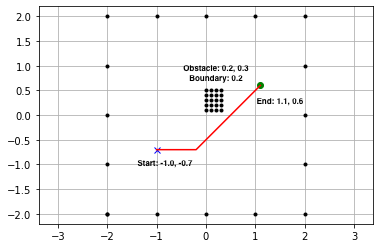
\includegraphics[scale=0.62]{images/img1.png}
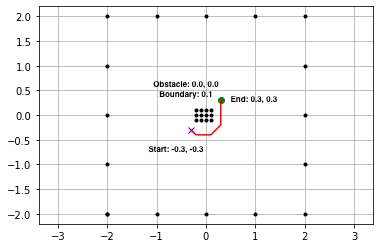
\includegraphics[scale=0.62]{images/img2.png}\\

After testing out quite a few paths and simulating them on Kuka, the experiment given in the assignment was carried out. The start point was chosen as $(-0.7, -0.7, 0.5)$ and the end point as $(1.1, 1.1, 0.5)$. The assignment states that the obstacle must be placed right in between these two points so, the obstacle was placed at $(0.2, 0.2, 0.5)$. \\
The path planning algorithm ran successfully and engendered the following path
\begin{figure}[h]
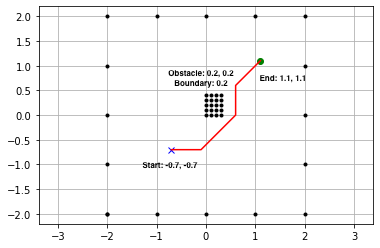
\includegraphics[scale=0.9]{images/img3.png}
\centering
\end{figure}
\newpage
This path was then fed into the end effector of a Kuka robot, which then using an IK control, successfully helped the end effector avoid the obstacle and reach its destination. The following pictures are screenshots of the actual motion of the arm in PyBullet.\\\\
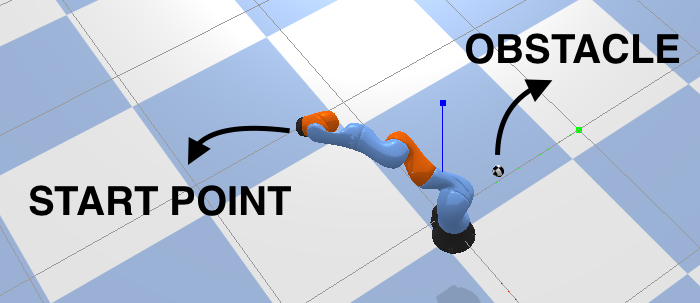
\includegraphics[scale=0.6]{images/img4.png}
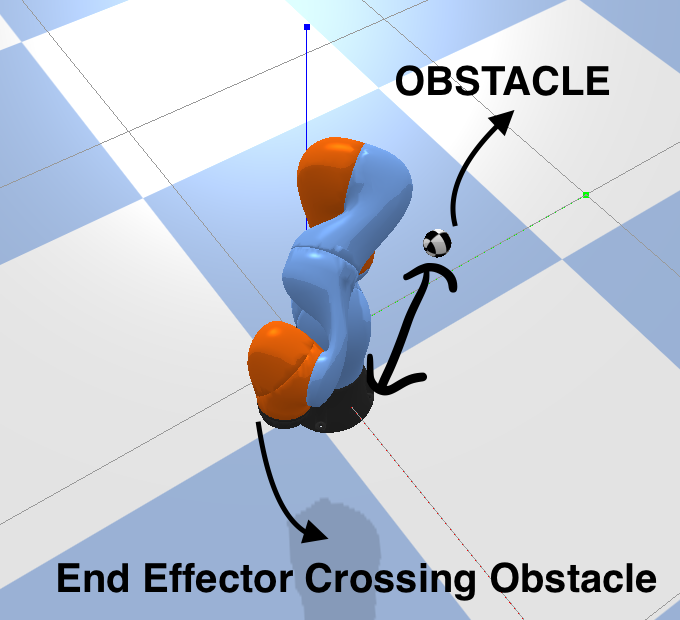
\includegraphics[scale=0.5]{images/img5.png}\\
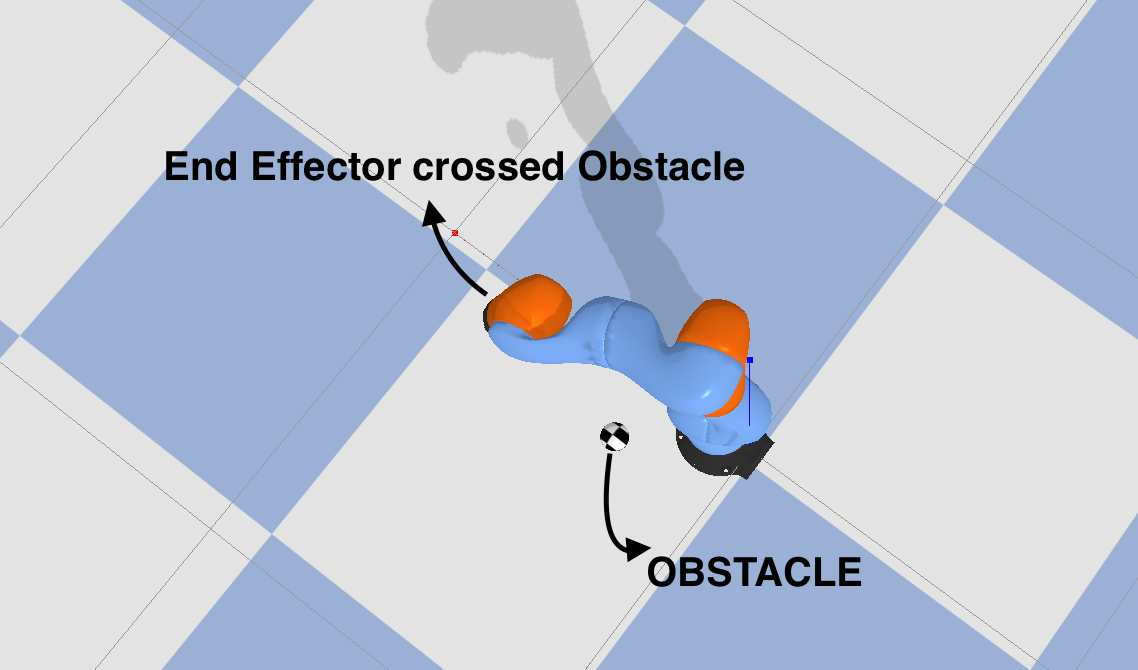
\includegraphics[scale=0.4]{images/img6.png}
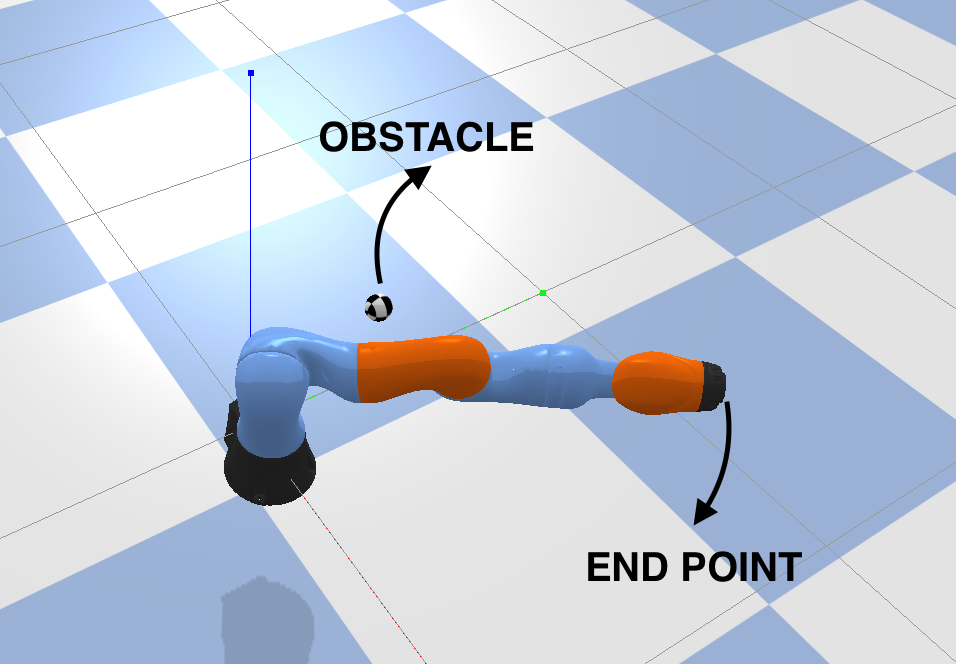
\includegraphics[scale=0.4]{images/img7.png}
\bigskip

\section{JUSTIFICATION}
The results from the experiments provide strong reasons to justify this approach. The code was able to predict an optimal path from the start to the end positions while avoiding the obstacle. It does not take a {\it complete-circle-around-the-obstacle} kind of approach but rather tries to determine the shortest possible path. When the {\it BoundaryCondition} is set as $1$, the algorithm knows to not go anywhere near 0.2 units of the obstacle which provides a guaranteed tolerance to any {\it reasonable} sudden disturbances that might otherwise cause the end effector to crash into the obstacle. The end effector always maintains at least 0.2 {\it(Boundary Conditions)} + 0.2 {\it(robot radius)} units of distance from the actual obstacle.\\

The path plots and screenshots in the previous section provide visual justification for the approach presented in this solution. A video demonstration of the code has also been uploaded to this Repo where the robot end effector successfully goes around the obstacle.
\bigskip

\section{LIMITATIONS}

This code runs well when the Z axis is set at 0.5 {\it(or any reasonable Z value)}. Following are a few limitations under the general setting and some solutions to overcome those - 
\begin{enumerate}
    \item If obstacle avoidance needs to be translated to a completely 3D problem, then there are two ways to proceed - One, the base code for the path finding algorithm needs to be updated to do a 3D grid based search rather than a 2D grid based search, or Two, the code can include a list variable Z {\it(for the Z axis, i.e. height)} that goes slightly above or below the obstacle whenever the end effector is near the obstacle. This variable can be used in conjecture with the current code and the end effector should be able to move around, avoiding obstacles anywhere in the 3D realm {\it(obviously, within the arm's reach)}
    \item The code does not plan the paths for all the other joints so it is possible that even when the end effector does not crash into the obstacle, the other parts of the arm still might - this has been currently prevented by using collision filters that will allow the arm to pass through the obstacle if it comes in contact
\end{enumerate}

\newpage

\section{REFERENCES}
\begin{enumerate}
    \item Sakai, A., Ingram, D., Dinius, J., Chawla, K., Raffin, A. and Paques, A., 2018. {\it PythonRobotics: a Python code collection of robotics algorithms}. arXiv preprint arXiv:1808.10703.
    \item Base code for Dijkstra's: {\it https://github.com/AtsushiSakai/PythonRobotics}
    \item Base code for PyBullet IK Sim: {\it https://github.com/McGIll-COMP-766-ECSE-683-Fall-2020/python-examples}
\end{enumerate}












%------------------------------------------------

\end{document}
